% Person 1 chapter. Included from main.tex with % Person 1 chapter. Included from main.tex with % Person 1 chapter. Included from main.tex with % Person 1 chapter. Included from main.tex with \input{sections/person1}.
% Replace every \textit{...} placeholder with your own text. Comment lines (%) do not appear in the PDF.
% Numbers: results/person1_riahana/summary.md and analysis.md.

\chapter{Raihana Grine}

\section{Methodology}
% - Task: decide whether a whole response is hallucinated; research question.
% - RoBERTa-base and DeBERTa-v3-base, pair input [context] [response], only the context is truncated.
% - Settings: 384 tokens, learning rate 2e-5, 3 epochs, batch size 16 through gradient accumulation,
%   8-bit AdamW; RoBERTa in fp16, DeBERTa in bfloat16; best epoch by validation macro-F1; seeds 42, 13, 2024.
% - Ablations and checks: response only, wrong context, cross-dataset, length and overlap baselines.
\textit{... The methodology used in this study ...}

\section{Experiments \& Findings}
% - Datasets, splits and label construction (see src/person1_riahana/README.md).
% - Main results, then ablations, significance tests, context sensitivity.
\textit{... The results of this study ...}

\input{tables/person1_results}

\begin{figure}[h]
    \centering
    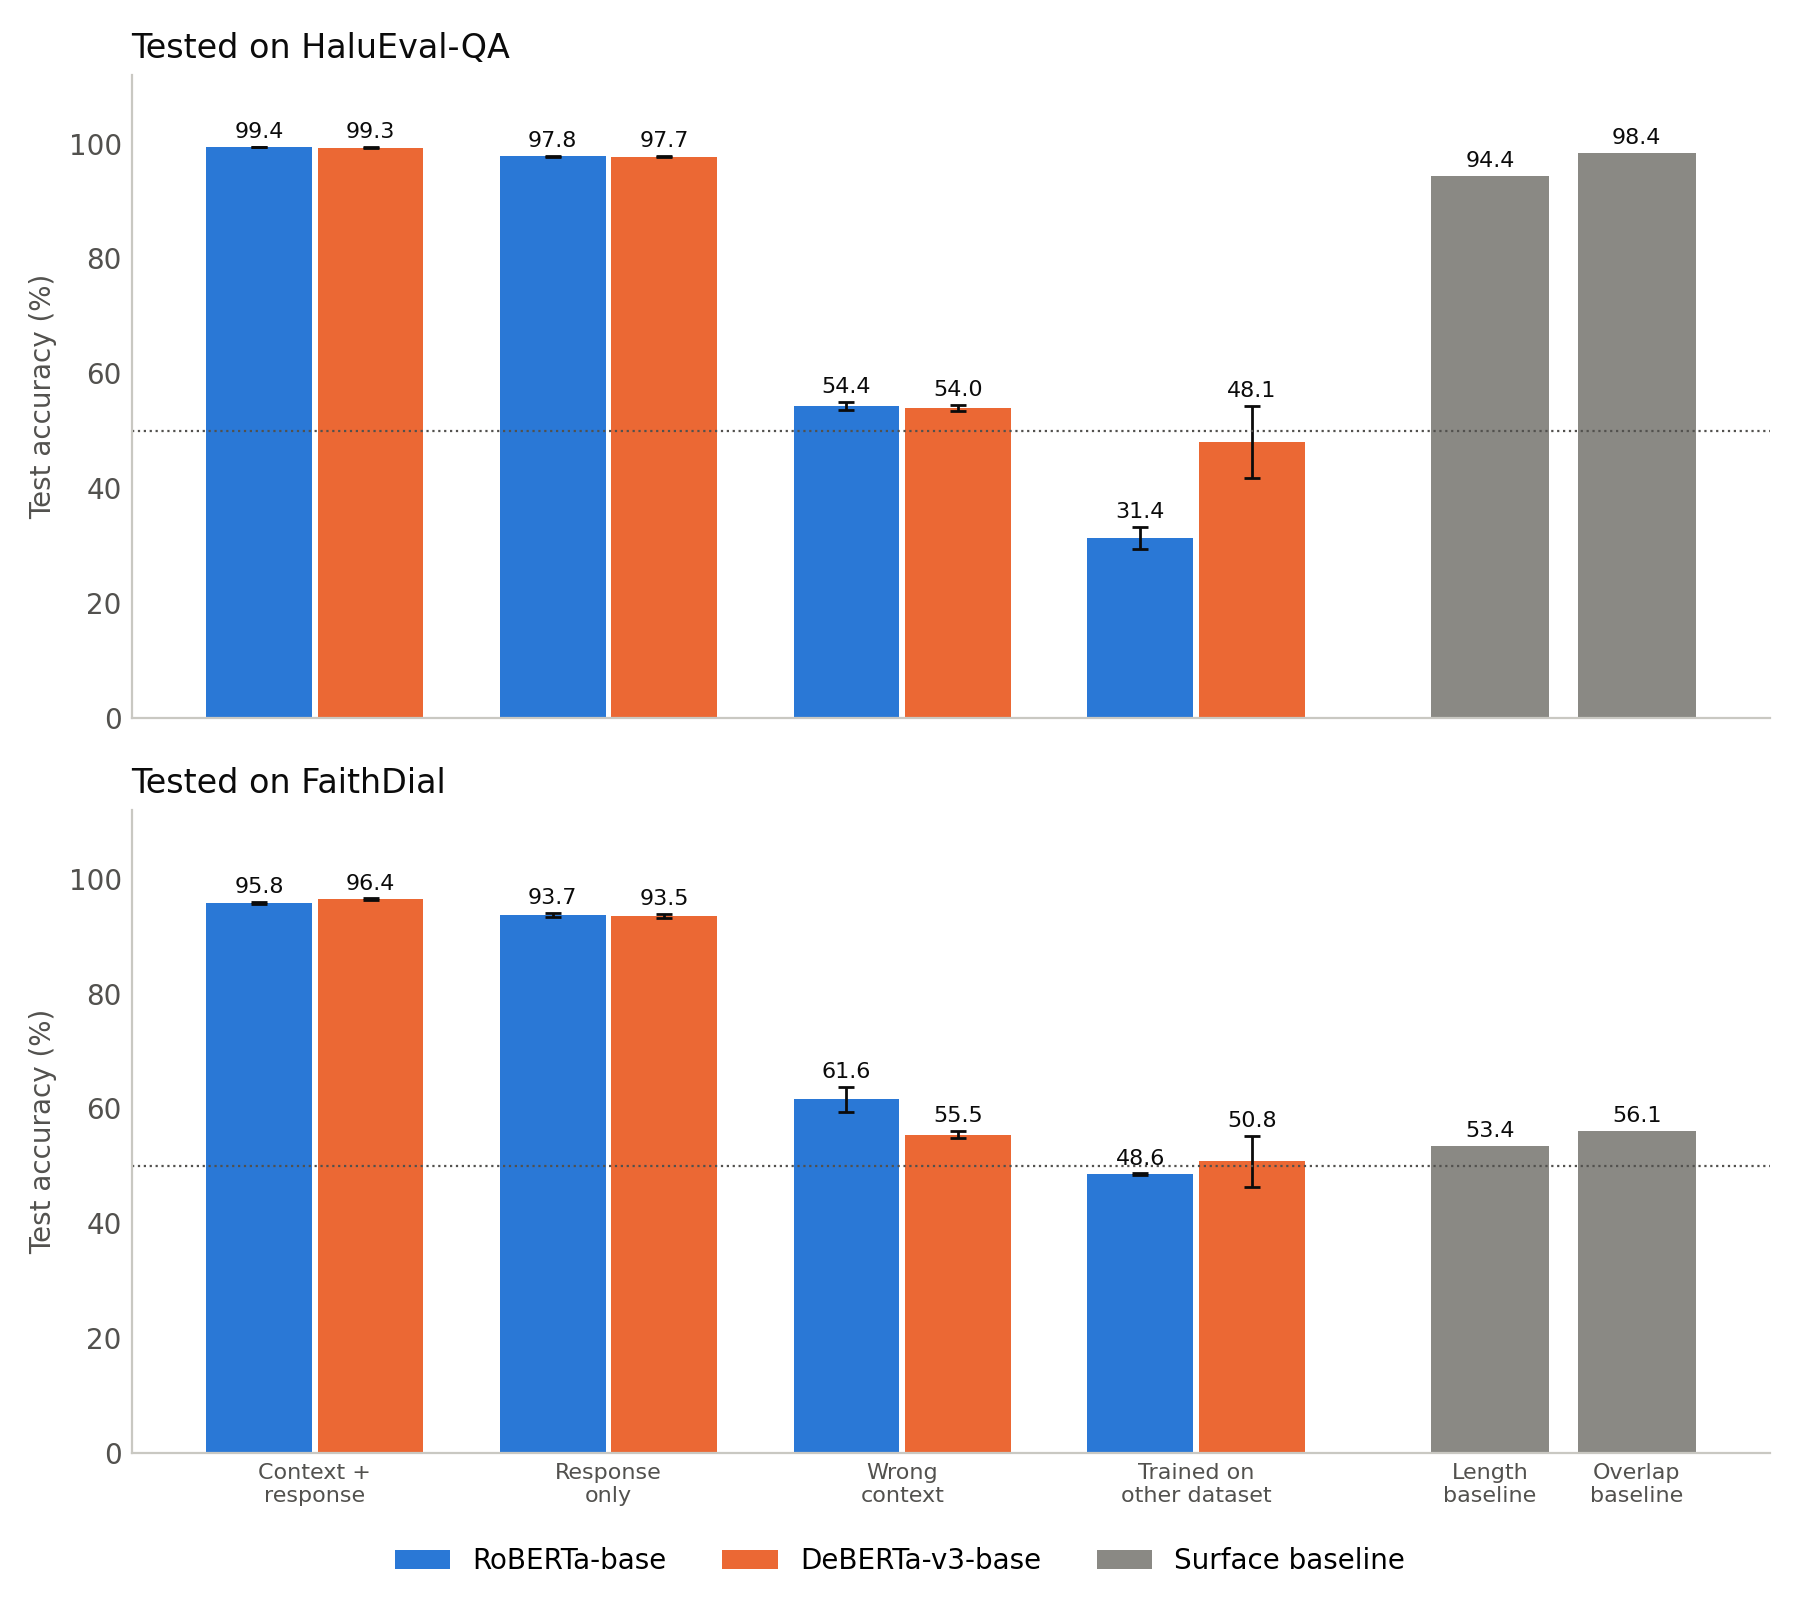
\includegraphics[width=\linewidth]{figures/person1/accuracy_by_setting.png}
    \caption{Test accuracy of both encoders in every setting, with the surface baselines. Error bars show the
    standard deviation over three training seeds.}
    \label{fig:p1-accuracy}
\end{figure}

\begin{figure}[h]
    \centering
    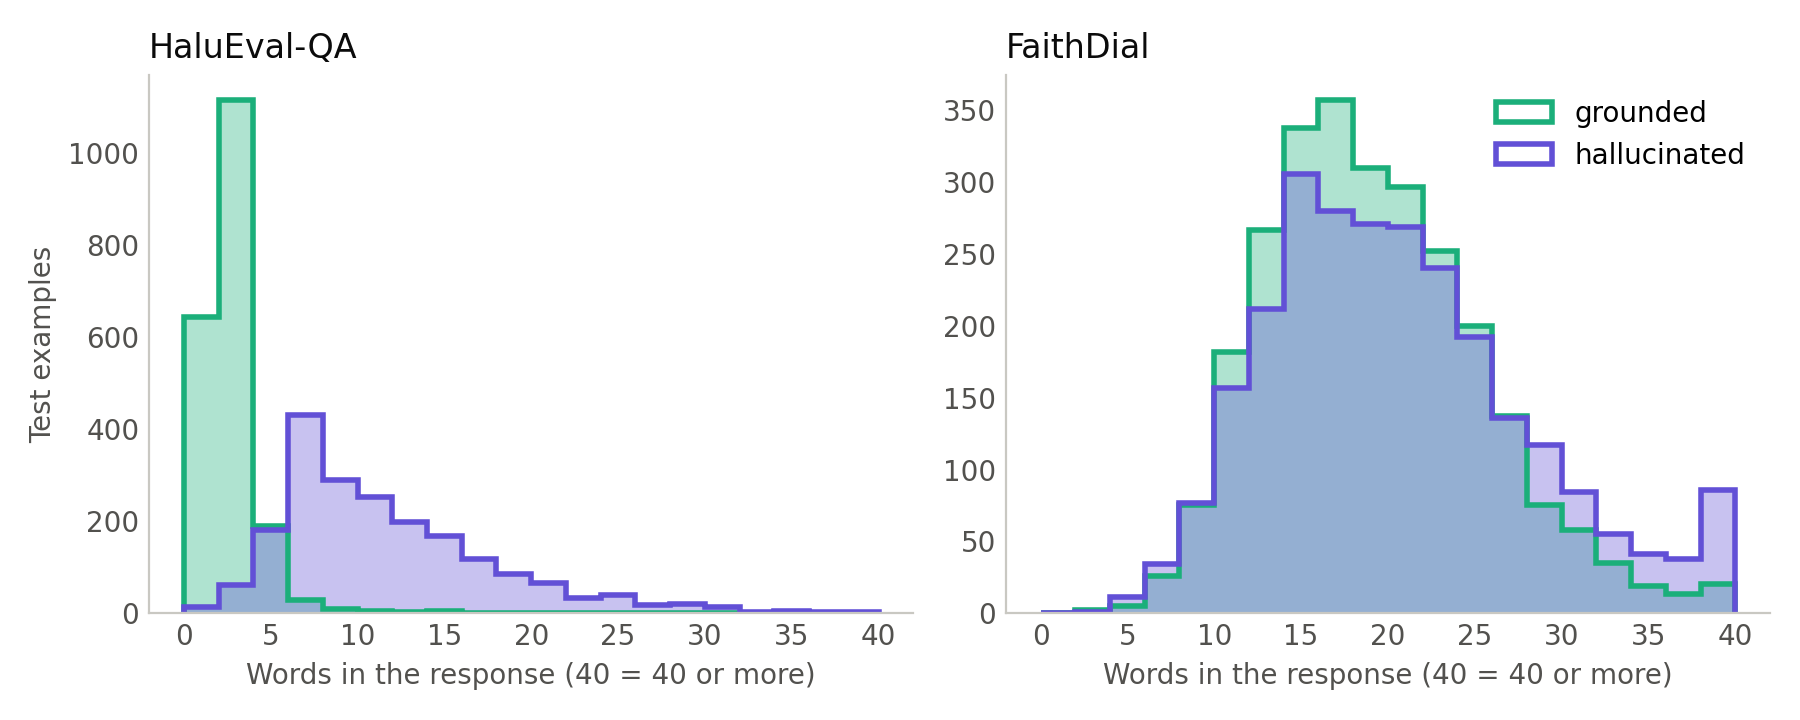
\includegraphics[width=\linewidth]{figures/person1/response_lengths.png}
    \caption{Response length of grounded and hallucinated test examples.}
    \label{fig:p1-lengths}
\end{figure}

\begin{figure}[h]
    \centering
    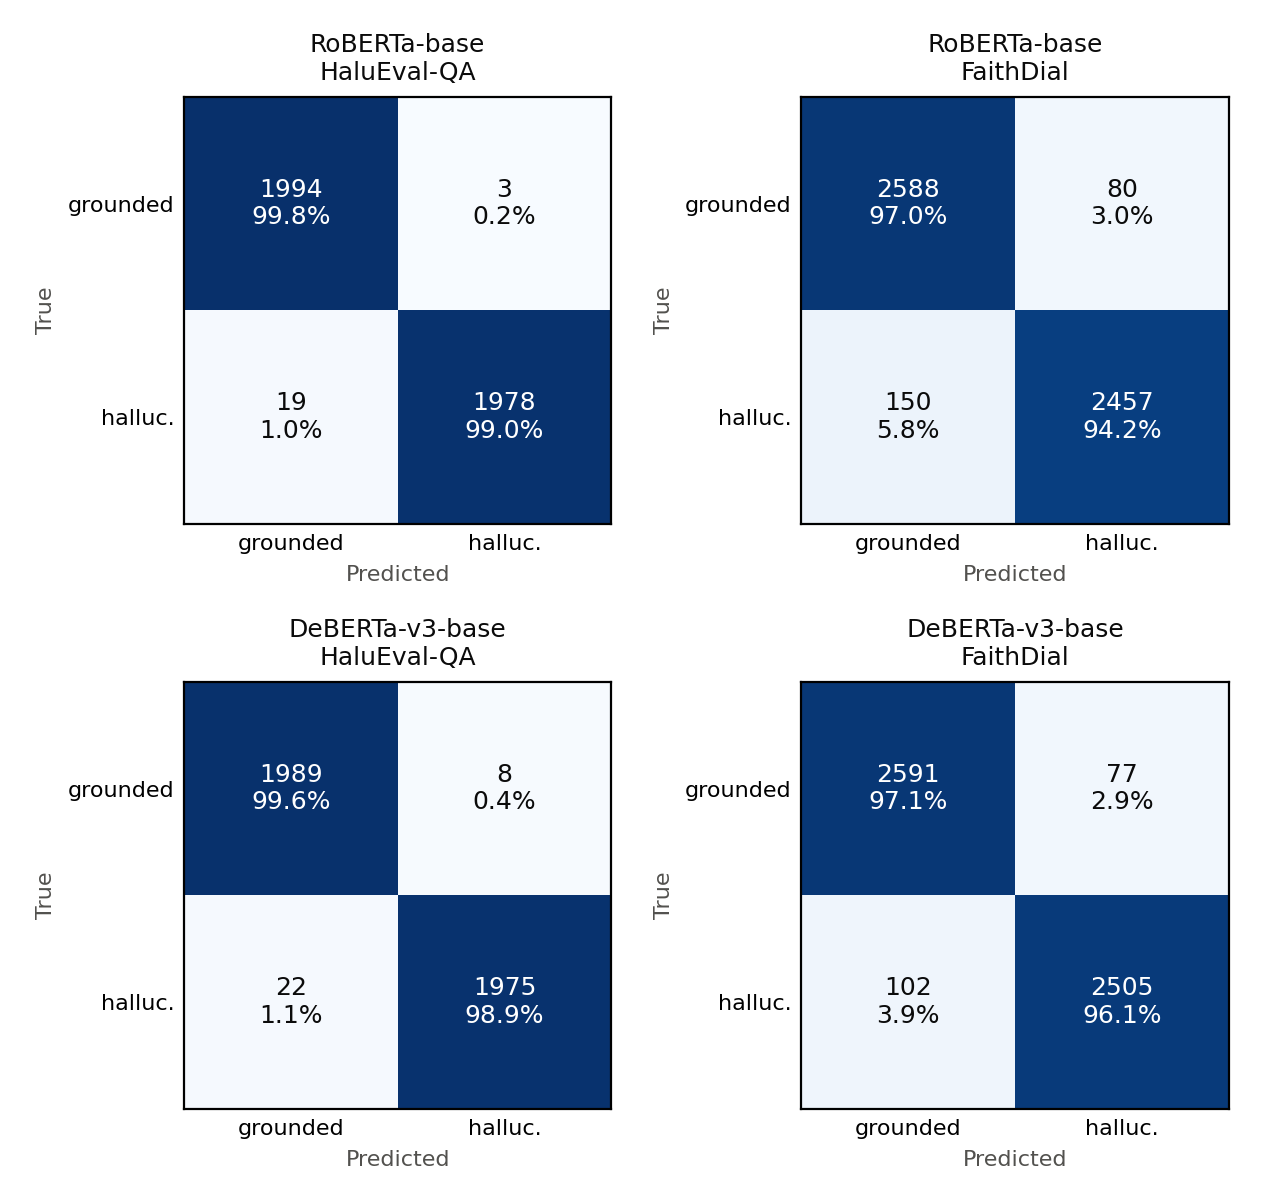
\includegraphics[width=.75\linewidth]{figures/person1/confusion_matrices.png}
    \caption{Confusion matrices of the full-input models on the test sets (seed 42).}
    \label{fig:p1-confusion}
\end{figure}

\section{Discussion}
% - Answer to the research question: grounding or shortcuts, with the evidence for both sides.
% - RoBERTa vs DeBERTa; why there is no transfer; hard examples.
% - Limitations: three seeds, data artefacts, different precision for the two models.
\textit{... The discussion for the results ...}

\section{Conclusion}
\textit{... The conclusion of this study ...}
.
% Replace every \textit{...} placeholder with your own text. Comment lines (%) do not appear in the PDF.
% Numbers: results/person1_riahana/summary.md and analysis.md.

\chapter{Raihana Grine}

\section{Methodology}
% - Task: decide whether a whole response is hallucinated; research question.
% - RoBERTa-base and DeBERTa-v3-base, pair input [context] [response], only the context is truncated.
% - Settings: 384 tokens, learning rate 2e-5, 3 epochs, batch size 16 through gradient accumulation,
%   8-bit AdamW; RoBERTa in fp16, DeBERTa in bfloat16; best epoch by validation macro-F1; seeds 42, 13, 2024.
% - Ablations and checks: response only, wrong context, cross-dataset, length and overlap baselines.
\textit{... The methodology used in this study ...}

\section{Experiments \& Findings}
% - Datasets, splits and label construction (see src/person1_riahana/README.md).
% - Main results, then ablations, significance tests, context sensitivity.
\textit{... The results of this study ...}

\begin{table}[h]
\centering
\resizebox{\textwidth}{!}{%
\begin{tabular}{lllcccc}
\hline
Dataset & Model & Setting & Acc & F1 & Macro-F1 & AUROC \\
\hline
HaluEval-QA & RoBERTa-base & Context + response & 0.994$\pm$0.000 & 0.994$\pm$0.000 & 0.994$\pm$0.000 & 0.998$\pm$0.000 \\
HaluEval-QA & DeBERTa-v3-base & Context + response & 0.993$\pm$0.001 & 0.993$\pm$0.001 & 0.993$\pm$0.001 & 0.998$\pm$0.001 \\
HaluEval-QA & RoBERTa-base & Response only & 0.978$\pm$0.001 & 0.977$\pm$0.001 & 0.978$\pm$0.001 & 0.989$\pm$0.001 \\
HaluEval-QA & DeBERTa-v3-base & Response only & 0.977$\pm$0.001 & 0.977$\pm$0.001 & 0.977$\pm$0.001 & 0.989$\pm$0.000 \\
HaluEval-QA & RoBERTa-base & Wrong context & 0.544$\pm$0.007 & 0.687$\pm$0.003 & 0.423$\pm$0.013 & 0.981$\pm$0.004 \\
HaluEval-QA & DeBERTa-v3-base & Wrong context & 0.540$\pm$0.005 & 0.685$\pm$0.002 & 0.417$\pm$0.009 & 0.883$\pm$0.116 \\
HaluEval-QA & RoBERTa-base & Trained on the other dataset & 0.314$\pm$0.019 & 0.458$\pm$0.032 & 0.260$\pm$0.010 & 0.368$\pm$0.013 \\
HaluEval-QA & DeBERTa-v3-base & Trained on the other dataset & 0.481$\pm$0.063 & 0.558$\pm$0.013 & 0.455$\pm$0.098 & 0.506$\pm$0.052 \\
HaluEval-QA & Baseline: length & Surface features only & 0.944 & 0.943 & 0.944 & 0.972 \\
HaluEval-QA & Baseline: overlap & Surface features only & 0.984 & 0.984 & 0.984 & 0.996 \\
\hline
FaithDial & RoBERTa-base & Context + response & 0.958$\pm$0.002 & 0.957$\pm$0.002 & 0.958$\pm$0.002 & 0.992$\pm$0.000 \\
FaithDial & DeBERTa-v3-base & Context + response & 0.964$\pm$0.002 & 0.963$\pm$0.002 & 0.964$\pm$0.002 & 0.994$\pm$0.000 \\
FaithDial & RoBERTa-base & Response only & 0.937$\pm$0.004 & 0.935$\pm$0.005 & 0.937$\pm$0.004 & 0.984$\pm$0.001 \\
FaithDial & DeBERTa-v3-base & Response only & 0.935$\pm$0.004 & 0.933$\pm$0.005 & 0.935$\pm$0.004 & 0.985$\pm$0.001 \\
FaithDial & RoBERTa-base & Wrong context & 0.616$\pm$0.022 & 0.720$\pm$0.011 & 0.554$\pm$0.034 & 0.942$\pm$0.024 \\
FaithDial & DeBERTa-v3-base & Wrong context & 0.555$\pm$0.006 & 0.689$\pm$0.003 & 0.452$\pm$0.011 & 0.921$\pm$0.017 \\
FaithDial & RoBERTa-base & Trained on the other dataset & 0.486$\pm$0.001 & 0.651$\pm$0.003 & 0.338$\pm$0.015 & 0.463$\pm$0.048 \\
FaithDial & DeBERTa-v3-base & Trained on the other dataset & 0.508$\pm$0.045 & 0.624$\pm$0.027 & 0.455$\pm$0.059 & 0.539$\pm$0.019 \\
FaithDial & Baseline: length & Surface features only & 0.534 & 0.519 & 0.534 & 0.548 \\
FaithDial & Baseline: overlap & Surface features only & 0.561 & 0.561 & 0.561 & 0.584 \\
\hline
\end{tabular}}
\caption{Test results of the response-level classifiers, their ablations and the surface baselines. F1 refers to the hallucinated class. Neural models are reported as mean $\pm$ standard deviation over the training seeds; the baselines are deterministic.}
\label{tab:p1-results}
\end{table}


\begin{figure}[h]
    \centering
    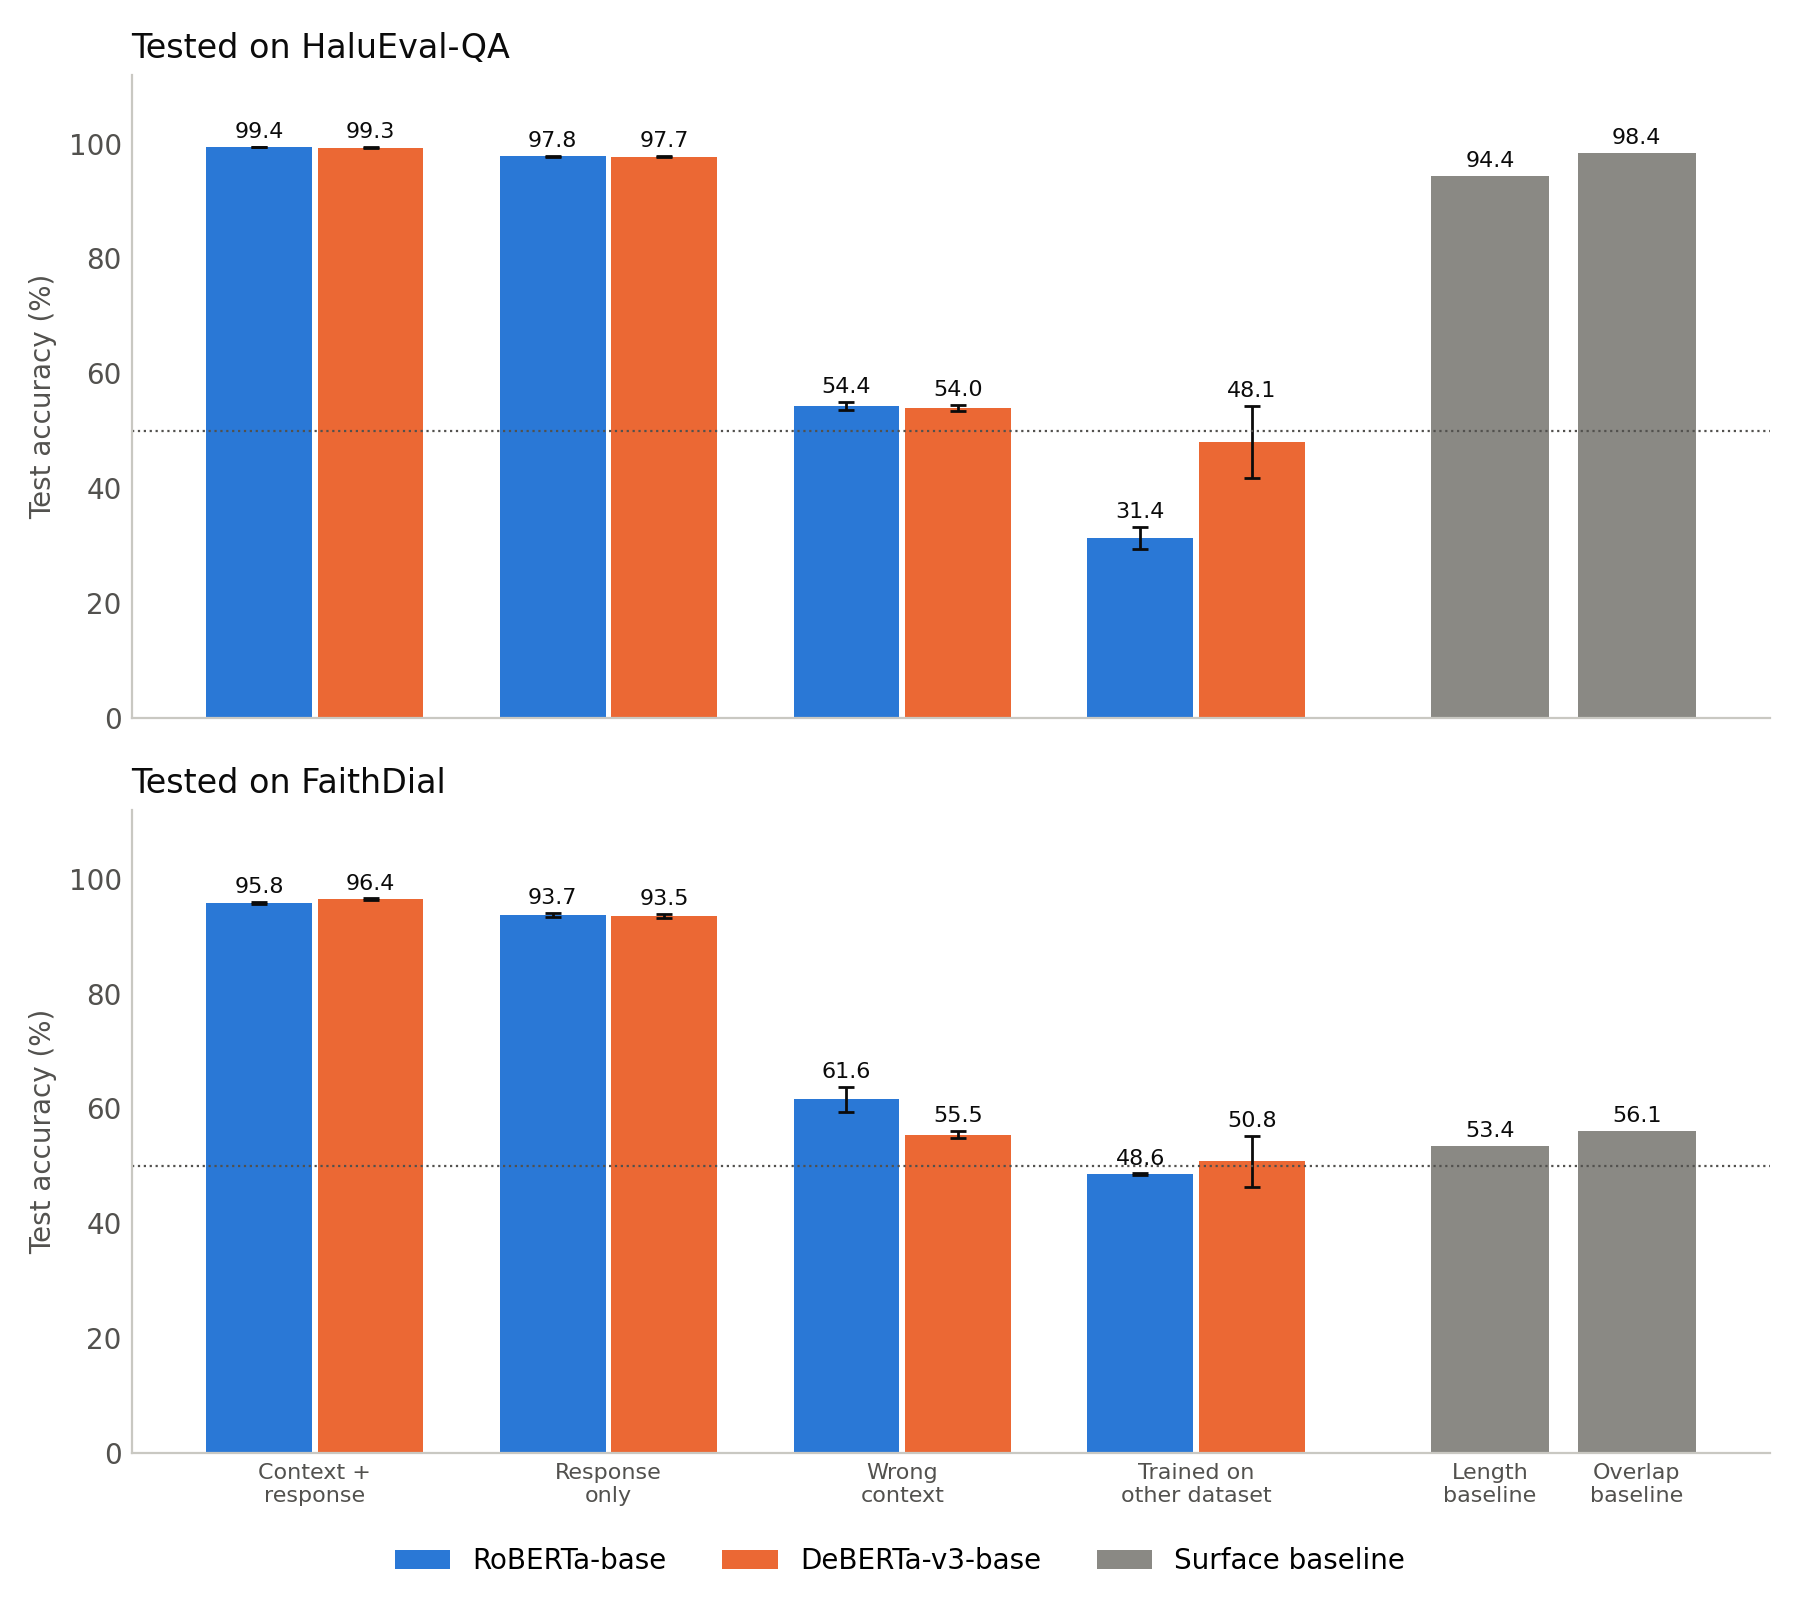
\includegraphics[width=\linewidth]{figures/person1/accuracy_by_setting.png}
    \caption{Test accuracy of both encoders in every setting, with the surface baselines. Error bars show the
    standard deviation over three training seeds.}
    \label{fig:p1-accuracy}
\end{figure}

\begin{figure}[h]
    \centering
    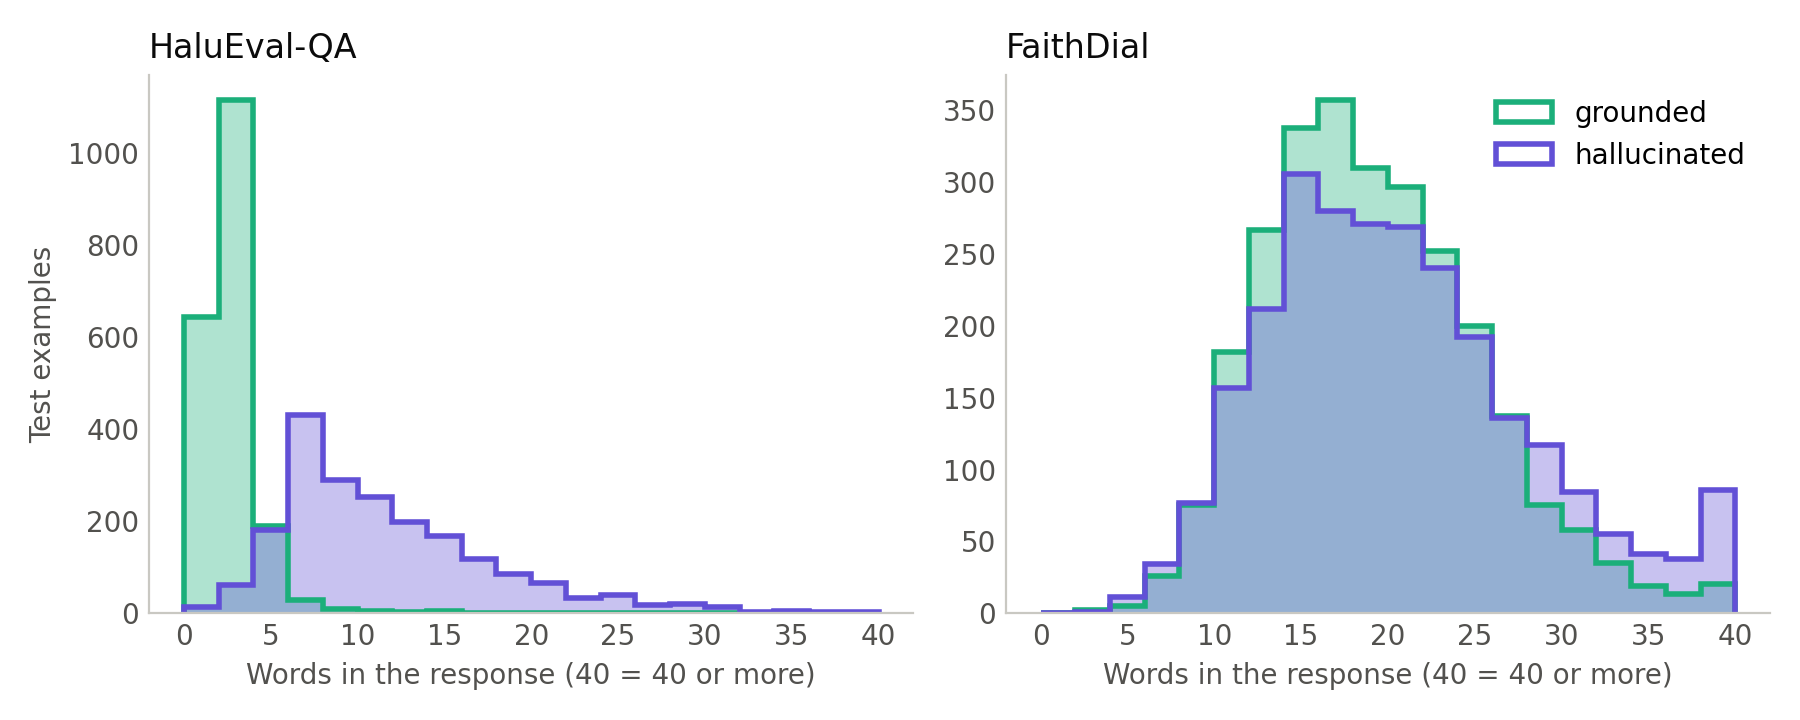
\includegraphics[width=\linewidth]{figures/person1/response_lengths.png}
    \caption{Response length of grounded and hallucinated test examples.}
    \label{fig:p1-lengths}
\end{figure}

\begin{figure}[h]
    \centering
    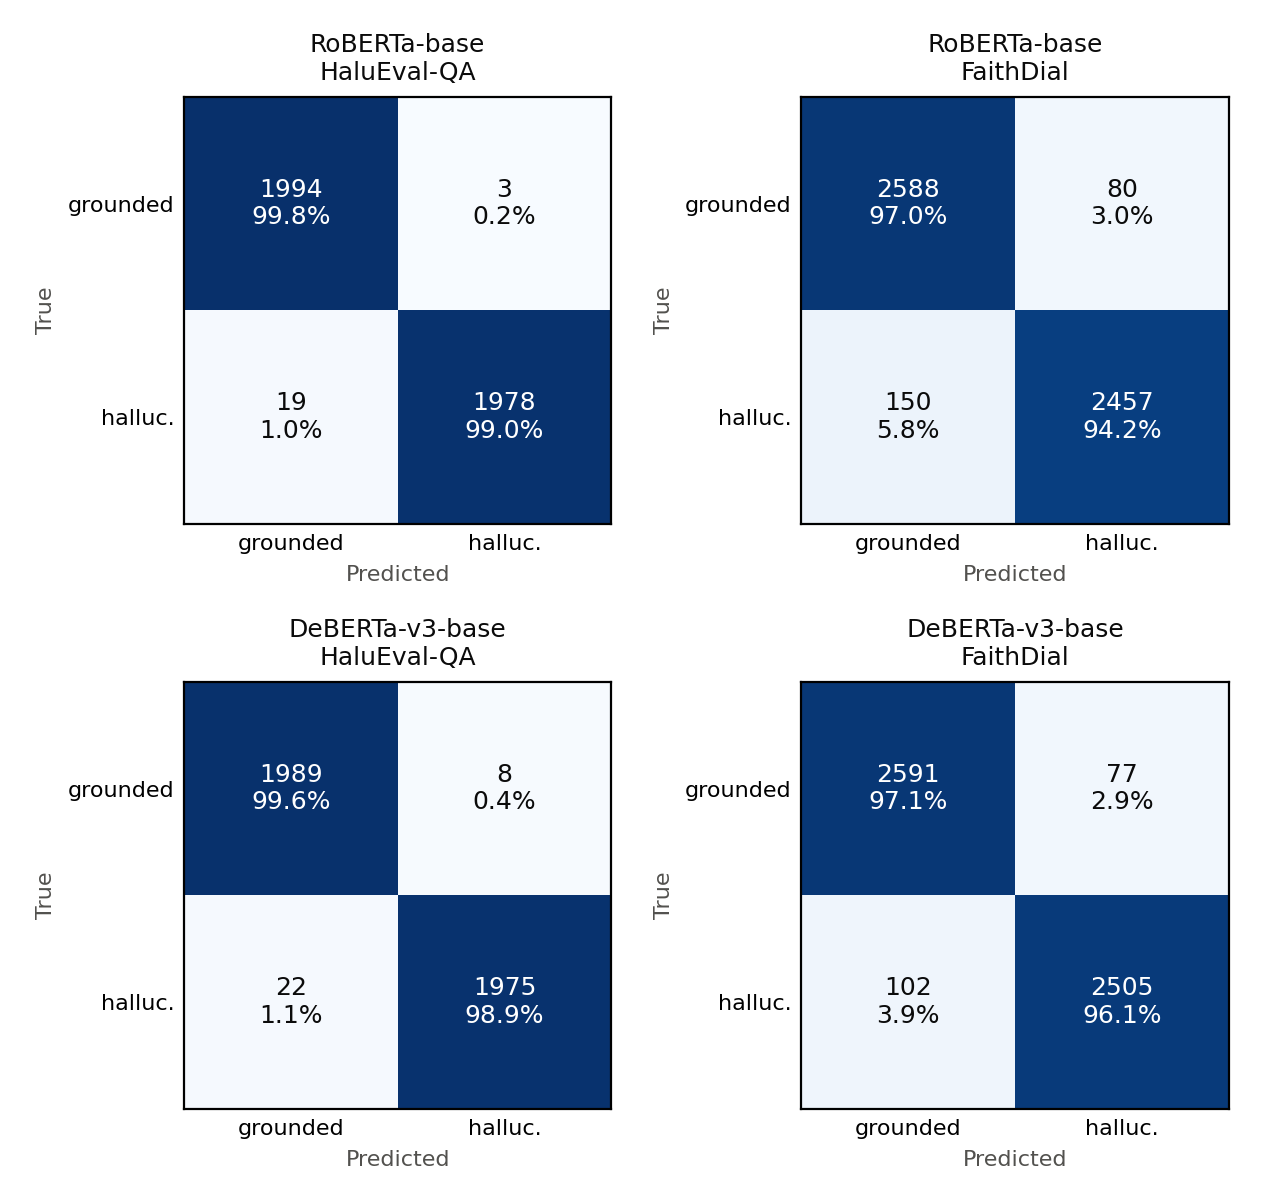
\includegraphics[width=.75\linewidth]{figures/person1/confusion_matrices.png}
    \caption{Confusion matrices of the full-input models on the test sets (seed 42).}
    \label{fig:p1-confusion}
\end{figure}

\section{Discussion}
% - Answer to the research question: grounding or shortcuts, with the evidence for both sides.
% - RoBERTa vs DeBERTa; why there is no transfer; hard examples.
% - Limitations: three seeds, data artefacts, different precision for the two models.
\textit{... The discussion for the results ...}

\section{Conclusion}
\textit{... The conclusion of this study ...}
.
% Replace every \textit{...} placeholder with your own text. Comment lines (%) do not appear in the PDF.
% Numbers: results/person1_riahana/summary.md and analysis.md.

\chapter{Raihana Grine}

\section{Methodology}
% - Task: decide whether a whole response is hallucinated; research question.
% - RoBERTa-base and DeBERTa-v3-base, pair input [context] [response], only the context is truncated.
% - Settings: 384 tokens, learning rate 2e-5, 3 epochs, batch size 16 through gradient accumulation,
%   8-bit AdamW; RoBERTa in fp16, DeBERTa in bfloat16; best epoch by validation macro-F1; seeds 42, 13, 2024.
% - Ablations and checks: response only, wrong context, cross-dataset, length and overlap baselines.
\textit{... The methodology used in this study ...}

\section{Experiments \& Findings}
% - Datasets, splits and label construction (see src/person1_riahana/README.md).
% - Main results, then ablations, significance tests, context sensitivity.
\textit{... The results of this study ...}

\begin{table}[h]
\centering
\resizebox{\textwidth}{!}{%
\begin{tabular}{lllcccc}
\hline
Dataset & Model & Setting & Acc & F1 & Macro-F1 & AUROC \\
\hline
HaluEval-QA & RoBERTa-base & Context + response & 0.994$\pm$0.000 & 0.994$\pm$0.000 & 0.994$\pm$0.000 & 0.998$\pm$0.000 \\
HaluEval-QA & DeBERTa-v3-base & Context + response & 0.993$\pm$0.001 & 0.993$\pm$0.001 & 0.993$\pm$0.001 & 0.998$\pm$0.001 \\
HaluEval-QA & RoBERTa-base & Response only & 0.978$\pm$0.001 & 0.977$\pm$0.001 & 0.978$\pm$0.001 & 0.989$\pm$0.001 \\
HaluEval-QA & DeBERTa-v3-base & Response only & 0.977$\pm$0.001 & 0.977$\pm$0.001 & 0.977$\pm$0.001 & 0.989$\pm$0.000 \\
HaluEval-QA & RoBERTa-base & Wrong context & 0.544$\pm$0.007 & 0.687$\pm$0.003 & 0.423$\pm$0.013 & 0.981$\pm$0.004 \\
HaluEval-QA & DeBERTa-v3-base & Wrong context & 0.540$\pm$0.005 & 0.685$\pm$0.002 & 0.417$\pm$0.009 & 0.883$\pm$0.116 \\
HaluEval-QA & RoBERTa-base & Trained on the other dataset & 0.314$\pm$0.019 & 0.458$\pm$0.032 & 0.260$\pm$0.010 & 0.368$\pm$0.013 \\
HaluEval-QA & DeBERTa-v3-base & Trained on the other dataset & 0.481$\pm$0.063 & 0.558$\pm$0.013 & 0.455$\pm$0.098 & 0.506$\pm$0.052 \\
HaluEval-QA & Baseline: length & Surface features only & 0.944 & 0.943 & 0.944 & 0.972 \\
HaluEval-QA & Baseline: overlap & Surface features only & 0.984 & 0.984 & 0.984 & 0.996 \\
\hline
FaithDial & RoBERTa-base & Context + response & 0.958$\pm$0.002 & 0.957$\pm$0.002 & 0.958$\pm$0.002 & 0.992$\pm$0.000 \\
FaithDial & DeBERTa-v3-base & Context + response & 0.964$\pm$0.002 & 0.963$\pm$0.002 & 0.964$\pm$0.002 & 0.994$\pm$0.000 \\
FaithDial & RoBERTa-base & Response only & 0.937$\pm$0.004 & 0.935$\pm$0.005 & 0.937$\pm$0.004 & 0.984$\pm$0.001 \\
FaithDial & DeBERTa-v3-base & Response only & 0.935$\pm$0.004 & 0.933$\pm$0.005 & 0.935$\pm$0.004 & 0.985$\pm$0.001 \\
FaithDial & RoBERTa-base & Wrong context & 0.616$\pm$0.022 & 0.720$\pm$0.011 & 0.554$\pm$0.034 & 0.942$\pm$0.024 \\
FaithDial & DeBERTa-v3-base & Wrong context & 0.555$\pm$0.006 & 0.689$\pm$0.003 & 0.452$\pm$0.011 & 0.921$\pm$0.017 \\
FaithDial & RoBERTa-base & Trained on the other dataset & 0.486$\pm$0.001 & 0.651$\pm$0.003 & 0.338$\pm$0.015 & 0.463$\pm$0.048 \\
FaithDial & DeBERTa-v3-base & Trained on the other dataset & 0.508$\pm$0.045 & 0.624$\pm$0.027 & 0.455$\pm$0.059 & 0.539$\pm$0.019 \\
FaithDial & Baseline: length & Surface features only & 0.534 & 0.519 & 0.534 & 0.548 \\
FaithDial & Baseline: overlap & Surface features only & 0.561 & 0.561 & 0.561 & 0.584 \\
\hline
\end{tabular}}
\caption{Test results of the response-level classifiers, their ablations and the surface baselines. F1 refers to the hallucinated class. Neural models are reported as mean $\pm$ standard deviation over the training seeds; the baselines are deterministic.}
\label{tab:p1-results}
\end{table}


\begin{figure}[h]
    \centering
    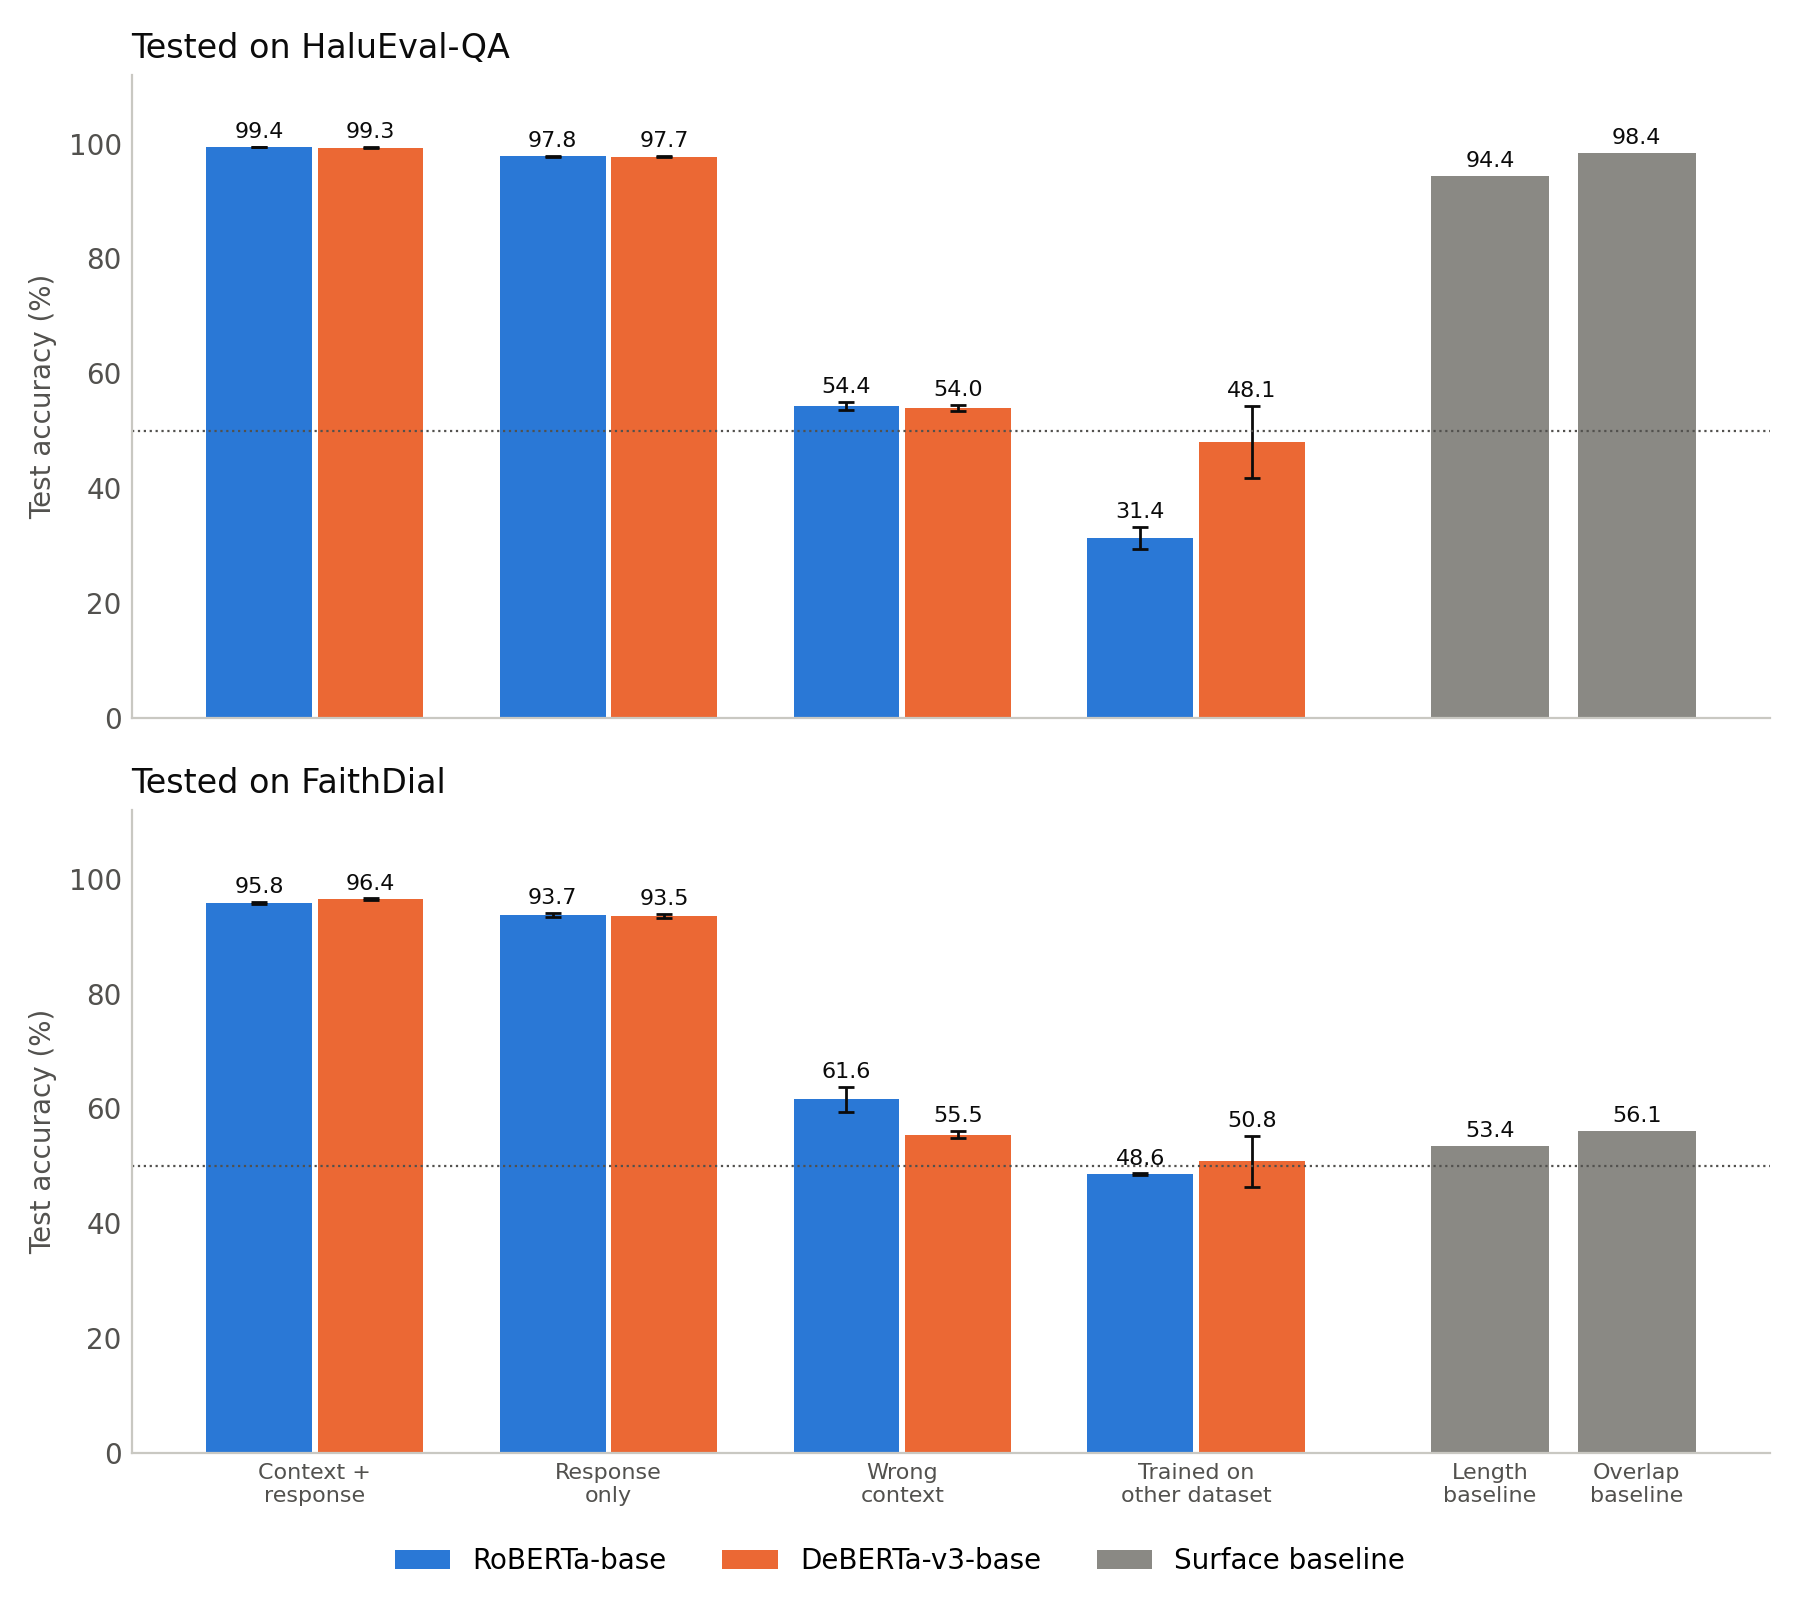
\includegraphics[width=\linewidth]{figures/person1/accuracy_by_setting.png}
    \caption{Test accuracy of both encoders in every setting, with the surface baselines. Error bars show the
    standard deviation over three training seeds.}
    \label{fig:p1-accuracy}
\end{figure}

\begin{figure}[h]
    \centering
    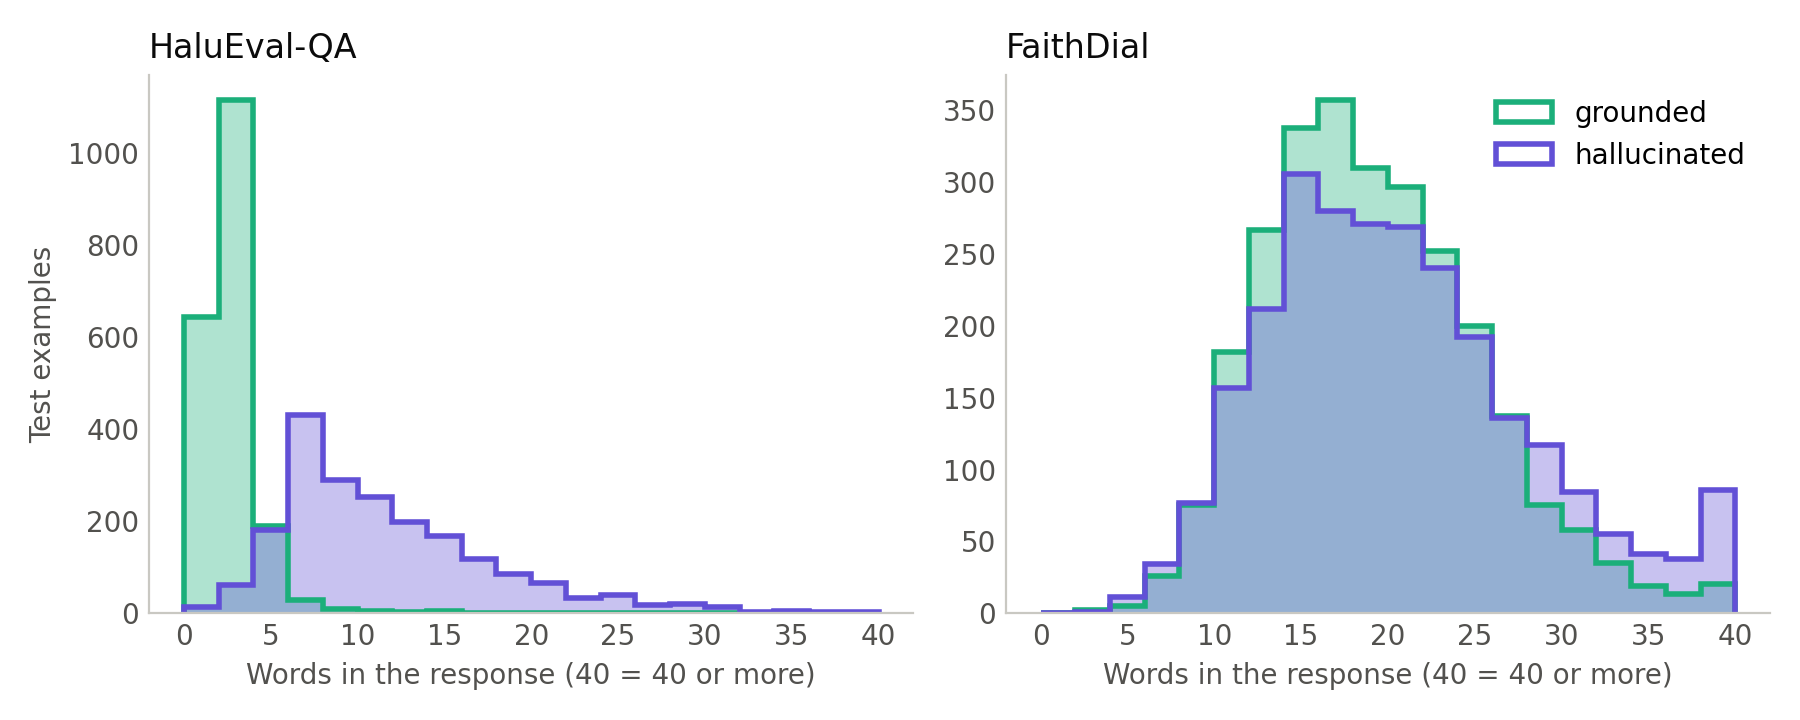
\includegraphics[width=\linewidth]{figures/person1/response_lengths.png}
    \caption{Response length of grounded and hallucinated test examples.}
    \label{fig:p1-lengths}
\end{figure}

\begin{figure}[h]
    \centering
    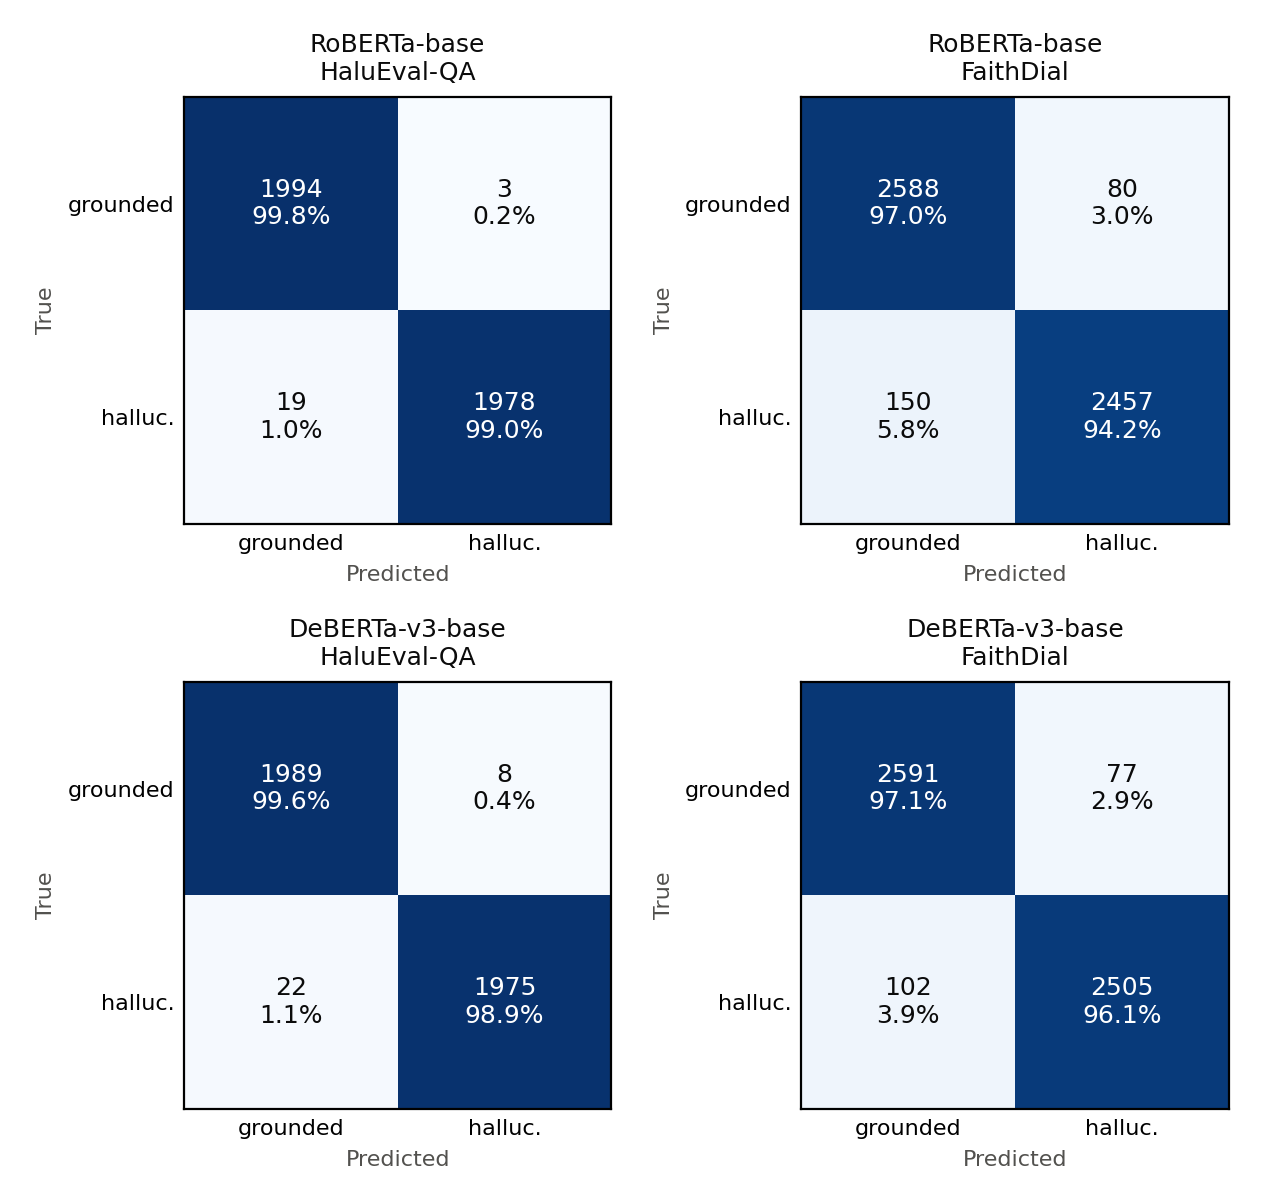
\includegraphics[width=.75\linewidth]{figures/person1/confusion_matrices.png}
    \caption{Confusion matrices of the full-input models on the test sets (seed 42).}
    \label{fig:p1-confusion}
\end{figure}

\section{Discussion}
% - Answer to the research question: grounding or shortcuts, with the evidence for both sides.
% - RoBERTa vs DeBERTa; why there is no transfer; hard examples.
% - Limitations: three seeds, data artefacts, different precision for the two models.
\textit{... The discussion for the results ...}

\section{Conclusion}
\textit{... The conclusion of this study ...}
.
% Replace every \textit{...} placeholder with your own text. Comment lines (%) do not appear in the PDF.
% Numbers: results/person1_riahana/summary.md and analysis.md.

\chapter{Raihana Grine}

\section{Methodology}
% - Task: decide whether a whole response is hallucinated; research question.
% - RoBERTa-base and DeBERTa-v3-base, pair input [context] [response], only the context is truncated.
% - Settings: 384 tokens, learning rate 2e-5, 3 epochs, batch size 16 through gradient accumulation,
%   8-bit AdamW; RoBERTa in fp16, DeBERTa in bfloat16; best epoch by validation macro-F1; seeds 42, 13, 2024.
% - Ablations and checks: response only, wrong context, cross-dataset, length and overlap baselines.
\textit{... The methodology used in this study ...}

\section{Experiments \& Findings}
% - Datasets, splits and label construction (see src/person1_riahana/README.md).
% - Main results, then ablations, significance tests, context sensitivity.
\textit{... The results of this study ...}

\begin{table}[h]
\centering
\resizebox{\textwidth}{!}{%
\begin{tabular}{lllcccc}
\hline
Dataset & Model & Setting & Acc & F1 & Macro-F1 & AUROC \\
\hline
HaluEval-QA & RoBERTa-base & Context + response & 0.994$\pm$0.000 & 0.994$\pm$0.000 & 0.994$\pm$0.000 & 0.998$\pm$0.000 \\
HaluEval-QA & DeBERTa-v3-base & Context + response & 0.993$\pm$0.001 & 0.993$\pm$0.001 & 0.993$\pm$0.001 & 0.998$\pm$0.001 \\
HaluEval-QA & RoBERTa-base & Response only & 0.978$\pm$0.001 & 0.977$\pm$0.001 & 0.978$\pm$0.001 & 0.989$\pm$0.001 \\
HaluEval-QA & DeBERTa-v3-base & Response only & 0.977$\pm$0.001 & 0.977$\pm$0.001 & 0.977$\pm$0.001 & 0.989$\pm$0.000 \\
HaluEval-QA & RoBERTa-base & Wrong context & 0.544$\pm$0.007 & 0.687$\pm$0.003 & 0.423$\pm$0.013 & 0.981$\pm$0.004 \\
HaluEval-QA & DeBERTa-v3-base & Wrong context & 0.540$\pm$0.005 & 0.685$\pm$0.002 & 0.417$\pm$0.009 & 0.883$\pm$0.116 \\
HaluEval-QA & RoBERTa-base & Trained on the other dataset & 0.314$\pm$0.019 & 0.458$\pm$0.032 & 0.260$\pm$0.010 & 0.368$\pm$0.013 \\
HaluEval-QA & DeBERTa-v3-base & Trained on the other dataset & 0.481$\pm$0.063 & 0.558$\pm$0.013 & 0.455$\pm$0.098 & 0.506$\pm$0.052 \\
HaluEval-QA & Baseline: length & Surface features only & 0.944 & 0.943 & 0.944 & 0.972 \\
HaluEval-QA & Baseline: overlap & Surface features only & 0.984 & 0.984 & 0.984 & 0.996 \\
\hline
FaithDial & RoBERTa-base & Context + response & 0.958$\pm$0.002 & 0.957$\pm$0.002 & 0.958$\pm$0.002 & 0.992$\pm$0.000 \\
FaithDial & DeBERTa-v3-base & Context + response & 0.964$\pm$0.002 & 0.963$\pm$0.002 & 0.964$\pm$0.002 & 0.994$\pm$0.000 \\
FaithDial & RoBERTa-base & Response only & 0.937$\pm$0.004 & 0.935$\pm$0.005 & 0.937$\pm$0.004 & 0.984$\pm$0.001 \\
FaithDial & DeBERTa-v3-base & Response only & 0.935$\pm$0.004 & 0.933$\pm$0.005 & 0.935$\pm$0.004 & 0.985$\pm$0.001 \\
FaithDial & RoBERTa-base & Wrong context & 0.616$\pm$0.022 & 0.720$\pm$0.011 & 0.554$\pm$0.034 & 0.942$\pm$0.024 \\
FaithDial & DeBERTa-v3-base & Wrong context & 0.555$\pm$0.006 & 0.689$\pm$0.003 & 0.452$\pm$0.011 & 0.921$\pm$0.017 \\
FaithDial & RoBERTa-base & Trained on the other dataset & 0.486$\pm$0.001 & 0.651$\pm$0.003 & 0.338$\pm$0.015 & 0.463$\pm$0.048 \\
FaithDial & DeBERTa-v3-base & Trained on the other dataset & 0.508$\pm$0.045 & 0.624$\pm$0.027 & 0.455$\pm$0.059 & 0.539$\pm$0.019 \\
FaithDial & Baseline: length & Surface features only & 0.534 & 0.519 & 0.534 & 0.548 \\
FaithDial & Baseline: overlap & Surface features only & 0.561 & 0.561 & 0.561 & 0.584 \\
\hline
\end{tabular}}
\caption{Test results of the response-level classifiers, their ablations and the surface baselines. F1 refers to the hallucinated class. Neural models are reported as mean $\pm$ standard deviation over the training seeds; the baselines are deterministic.}
\label{tab:p1-results}
\end{table}


\begin{figure}[h]
    \centering
    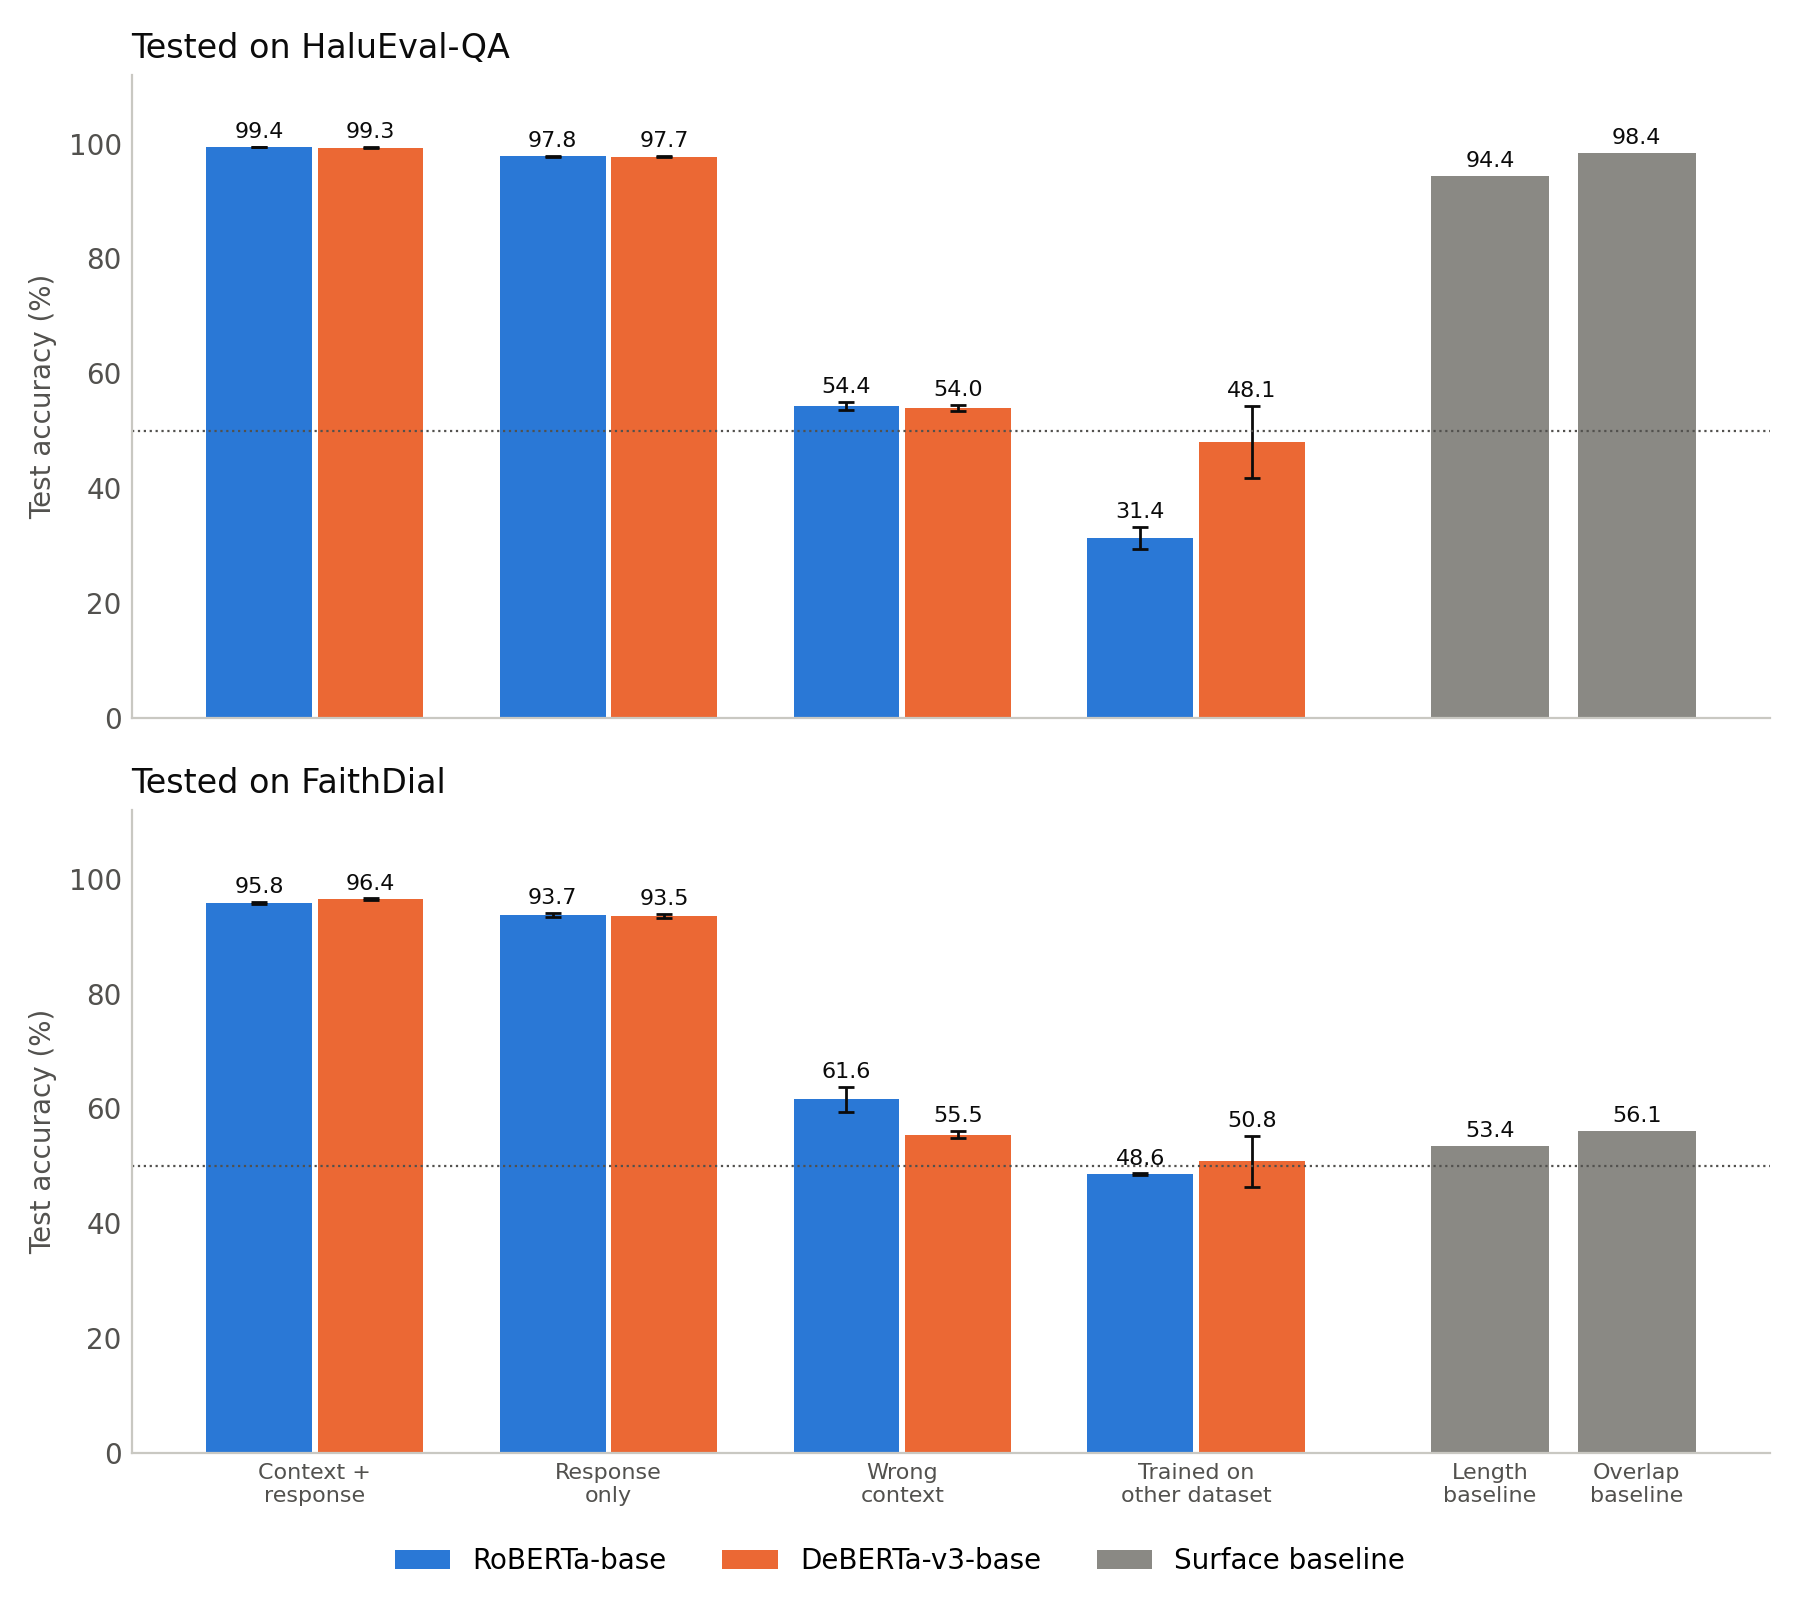
\includegraphics[width=\linewidth]{figures/person1/accuracy_by_setting.png}
    \caption{Test accuracy of both encoders in every setting, with the surface baselines. Error bars show the
    standard deviation over three training seeds.}
    \label{fig:p1-accuracy}
\end{figure}

\begin{figure}[h]
    \centering
    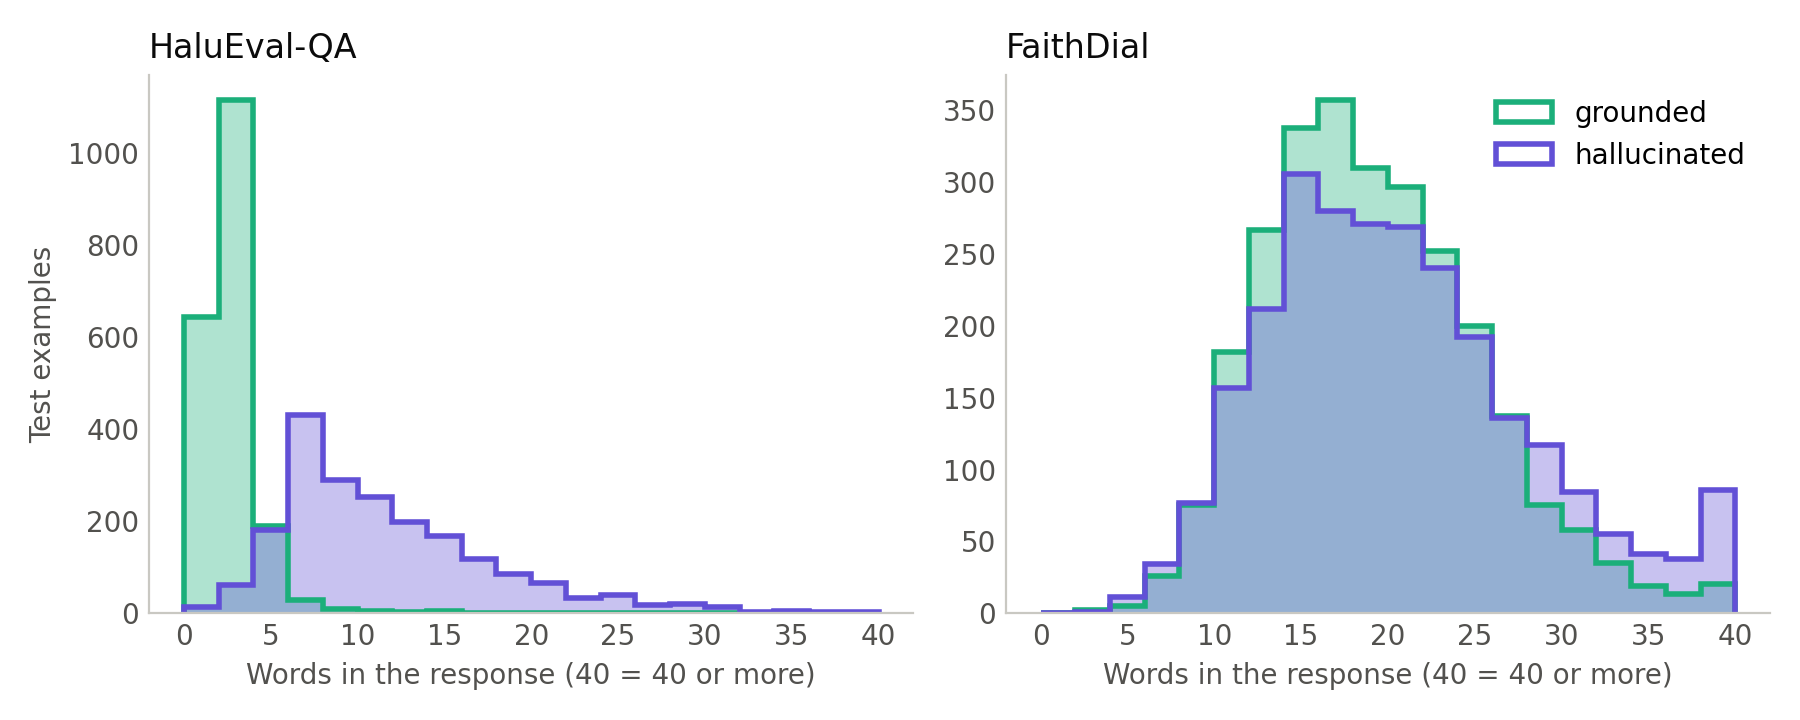
\includegraphics[width=\linewidth]{figures/person1/response_lengths.png}
    \caption{Response length of grounded and hallucinated test examples.}
    \label{fig:p1-lengths}
\end{figure}

\begin{figure}[h]
    \centering
    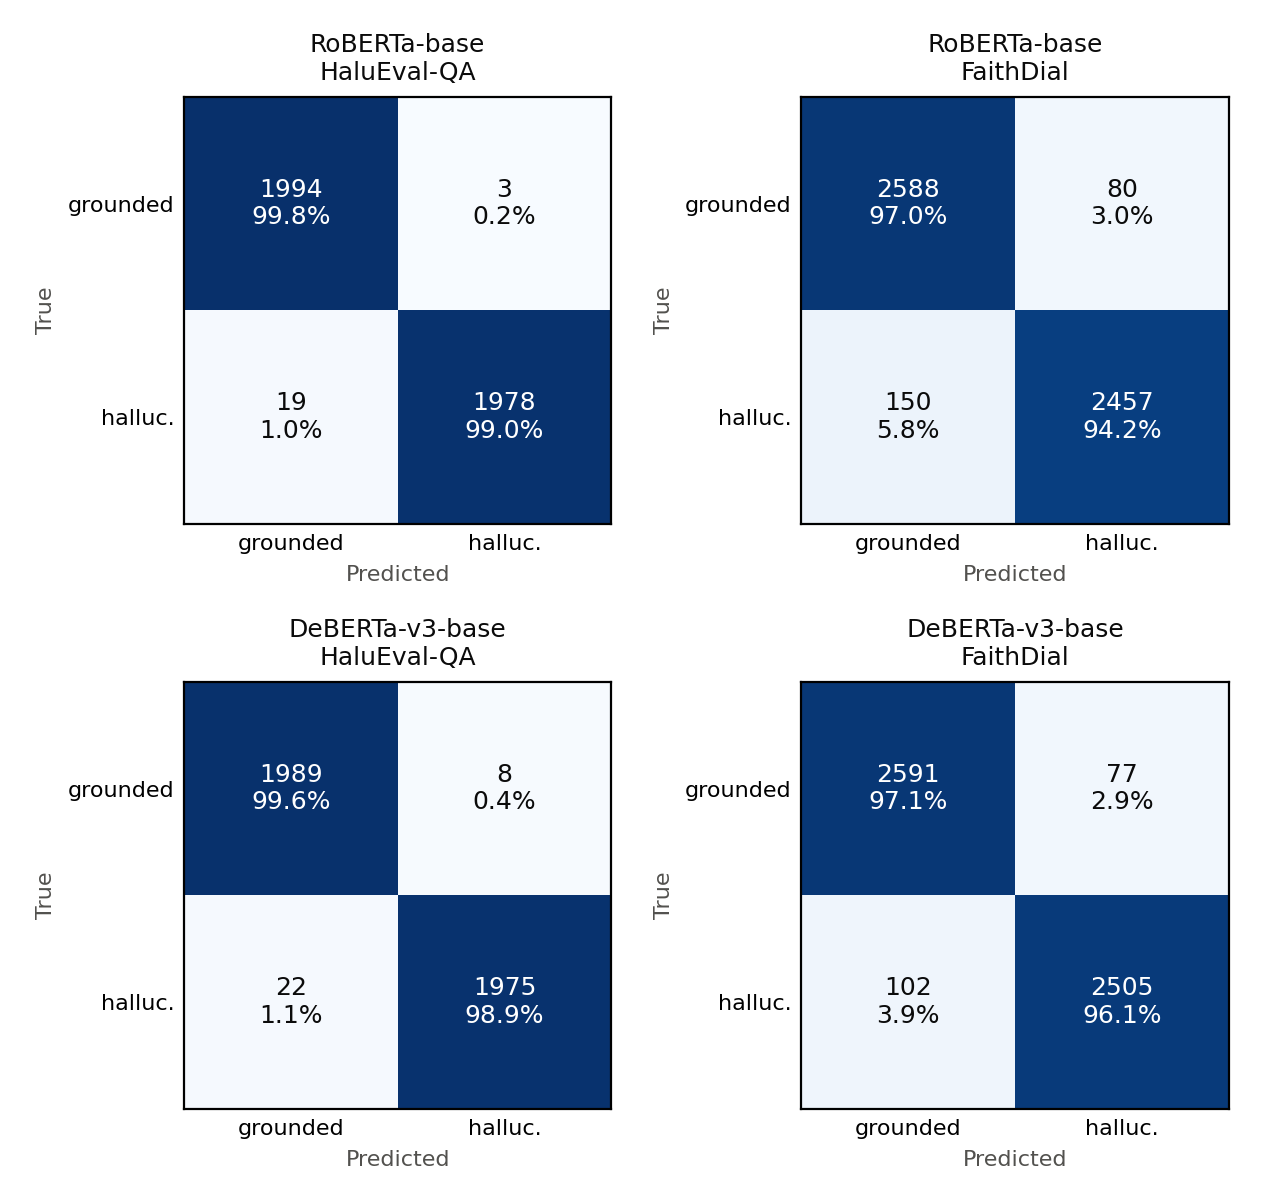
\includegraphics[width=.75\linewidth]{figures/person1/confusion_matrices.png}
    \caption{Confusion matrices of the full-input models on the test sets (seed 42).}
    \label{fig:p1-confusion}
\end{figure}

\section{Discussion}
% - Answer to the research question: grounding or shortcuts, with the evidence for both sides.
% - RoBERTa vs DeBERTa; why there is no transfer; hard examples.
% - Limitations: three seeds, data artefacts, different precision for the two models.
\textit{... The discussion for the results ...}

\section{Conclusion}
\textit{... The conclusion of this study ...}
